% Source ID: src-c47985c709ff8ae42e6e192879d604223c58a53c4358056d28f78ad5a9736e3c
% Source PDF SHA-256: a33455d27abdf2c4b344a5b90395bd71269f6fbefdef350375aba074e47ef700
% Source page 1 (printed page 943), question 13. Gray fill is the source's shaded set.
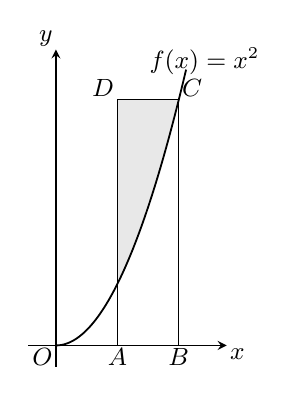
\begin{tikzpicture}[
  x=0.78cm,
  y=0.78cm,
  >=stealth,
  every node/.style={font=\small,inner sep=1pt},
  line width=0.45pt
]
\fill[gray!18] (1,1)--(1,4)--(2,4)
  plot[domain=2:1,samples=60] (\x,{\x*\x})--cycle;

\draw[->] (-0.45,0)--(2.78,0) node[below right] {$x$};
\draw[->] (0,-0.35)--(0,4.82) node[above left] {$y$};
\draw (1,0)--(1,4)--(2,4)--(2,0);
\draw[line width=0.65pt] plot[domain=0:2.12,samples=80] (\x,{\x*\x});

\node[below left] at (0,0) {$O$};
\node[below] at (1,0) {$A$};
\node[below] at (2,0) {$B$};
\node[above left] at (1,4) {$D$};
\node[above right] at (2,4) {$C$};
\node[above right] at (1.47,4.35) {$f(x)=x^2$};
\end{tikzpicture}
